\documentclass[sigconf,screen]{acmart}
\usepackage{tikz}
\usetikzlibrary{arrows}
\tikzset{
  big dot/.style={
    circle, inner sep=0pt, 
    minimum size=3pt, fill=purple
 }
}
\tikzset{
  bigbig dot/.style={
    circle, inner sep=0pt, 
    minimum size=5pt, fill=purple
 }
}
\tikzset{
  bigorange dot/.style={
    circle, inner sep=0pt, 
    minimum size=2.5pt, fill=orange
 }
}
\usetikzlibrary{decorations.pathmorphing}
\usetikzlibrary{decorations.pathreplacing}
\tikzset{snake it/.style={decorate, decoration=snake}}

\begin{document}

  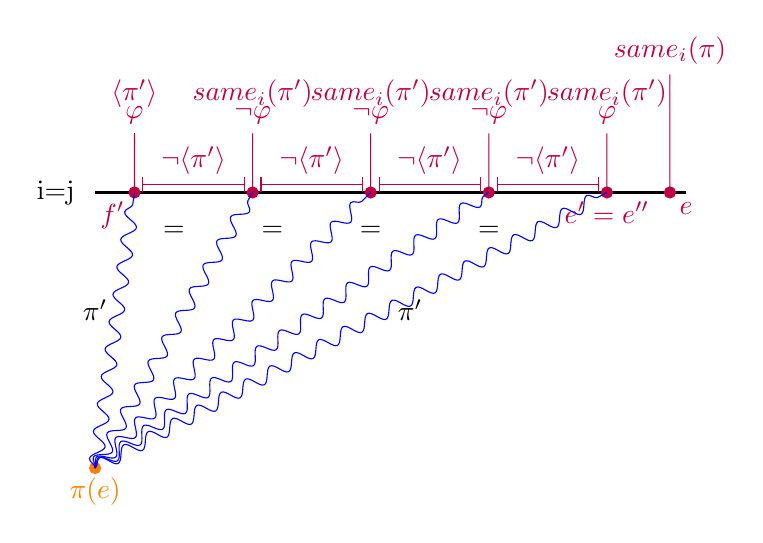
\begin{tikzpicture}
    \node at (0,4) {i=j};
    \draw[black, very thick] (0.5,4) -- (8,4);




    \draw (1,4) to (1,4.75);
    \filldraw[orange] (0.5,0.5) circle (2pt) node[anchor=north]{$\pi(e)$};
    \filldraw[purple] (1,4) circle (2pt) node[anchor=north east]{$f'$} to (1,4.75) node[anchor=south]{$\varphi$} (1,5.25) node[]{$\langle\pi'\rangle$};
    \filldraw[purple] (7,4) circle (2pt) node[anchor=north]{$e'=e''$} to (7,4.75) node[anchor=south]{$\varphi$} (7,5.25) node[]{$same_{i}(\pi')$};
    \filldraw[purple] (5.5,4) circle (2pt) node[anchor=north]{} to (5.5,4.75) node[anchor=south]{$\lnot \varphi$} (5.5,5.25) node[]{$same_{i}(\pi')$};
    \filldraw[purple] (4,4) circle (2pt) node[anchor=north]{} to (4,4.75) node[anchor=south]{$\lnot \varphi$} (4,5.25) node[]{$same_{i}(\pi')$};
    \filldraw[purple] (2.5,4) circle (2pt) node[anchor=north]{} to (2.5,4.75) node[anchor=south]{$\lnot \varphi$} (2.5,5.25) node[]{$same_{i}(\pi')$};
     \filldraw[purple] (7.8,4) circle (2pt) node[anchor=north west]{$e$} to (7.8,5.5) node[anchor=south]{$same_{i}(\pi)$};





    \path [draw=blue,snake it] (0.5,0.5)--(1,4) (0.5,2.50) node{$\pi'$};
   \path [draw=blue,snake it] (0.5,0.5)--(7,4) (1.5,3.5) node{$=$};
   \path [draw=blue,snake it] (0.5,0.5)--(5.5,4) (2.75,3.50) node{$=$};
   \path [draw=blue,snake it] (0.5,0.5)--(4,4) (4,3.50) node{$=$};
   \path [draw=blue,snake it] (0.5,0.5)--(2.5,4) (5.5,3.50) node{$=$} (4.5,2.5) node {$\pi'$};

\draw[|-|,draw=purple] (1.1,4.1) -- (2.4,4.1) node[text =purple,midway, anchor=south]{$\lnot \langle\pi'\rangle$};
\draw[|-|,draw=purple] (2.6,4.1) -- (3.9,4.1) node[text =purple,midway, anchor=south]{$\lnot \langle\pi'\rangle$};
\draw[|-|,draw=purple] (4.1,4.1) -- (5.4,4.1) node[text =purple,midway, anchor=south]{$\lnot \langle\pi'\rangle$};
\draw[|-|,draw=purple] (5.6,4.1) -- (6.9,4.1) node[text =purple,midway, anchor=south]{$\lnot \langle\pi'\rangle$};

\end{tikzpicture}

\end{document}